\chapter{Server}
Il passaggio principale che ho dovuto affrontare per l'inizio del progetto è stata l'inizializzazione
di un server che potesse gestire lo scambio di informazioni con l'applicazione ed occuparsi di svolgere tutte i compiti del caso.

Il lavoro del server è facilmente scomponibile in due parti, la gestione dei dati utili per la classificazione 
(che sarà poi affrontata nel capitolo \ref{chapter:classification}) e l'erogazione di dati informativi che vedremo consentire
ad un amministratore l'interazione con il sistema.

Si è scelto di sviluppare il tutto con il linguaggio Python e di inserire per comodità il software in due differenti contenitori Docker, in modo da 
mantenere differenziate queste due parti anche a livello programmativo.

\subsubsection{Docker}
Docker \cite{docker} è un progetto open-source in grado di effettuare il deploy di applicazioni all'interno di contenitori software che grazie alla
virtualizzazione si trovano ad un livello di astrazione differente dal sistema host. Questa tecnica è molto utile quando si vuole
mantenere separati l'installazione di un'applicativo dal sistema ospitante.



\section{RESTful Web API}
\label{section:api}
Come si intuisce in figura \ref{fig:overview}, si è pensato alla creazione di una RESTful Web API, ovvero interfaccia composta da un insieme
di \textit{endpoints} pubblici che consentono di ottenere delle informazioni mediante un sistema di richiesta-risposta tra client e server.

Tutti i componenti dell'app e del classificatore interessati a tali informazioni sono in grado di ricavarle con richieste a queste API, il che 
consente di avere accesso ad informazioni sempre aggiornate. Un cambiamento dei valori in fase di amministrazione consentirà la 
distribuzione delle modifiche senza la necessità del rilascio di un'aggiornamento dell'applicazione o riprogrammazione del ricevitore.


\subsection{Protocollo e formato}
Tutte le richieste e le risposte utilizzando per lo scambio dati il protocollo HTTP, il comune protocollo di livello 
applicativo utilizzato nel World Wide Web.

I dati sono trasmessi con il formato JSON, un formato standard che sfrutta una notazione chiave-valore facilmente leggibile.


\subsection{Endpoints}
Gli endpoints sono i punti in cui un software esterno accede a determinate informazioni. L'accesso avviene mediante la chiamata ad un URL 
web che ci si aspetta risponda con i dati richiesti.

\subsubsection{Lista delle attività}
Il primo degli endpoints impostato riguarda la lista di tutte le attività che il sistema imparerà a riconoscere.
Ogni attività conterrà
\begin{itemize}
    \item l'identificativo numerico
    \item il nome
    \item le traduzioni nelle lingue ammesse
    \item il tempo (in secondi) indicante la durata necessaria per l'addestramento dell'attività
\end{itemize}

\begin{listing}[H] 
    \begin{minted}[frame=single,framesep=10pt]{text}
        http://IP_ADDRESS:PORT/activities
    \end{minted}
    \caption{Endpoint per la lista delle attività}
    \label{listing:endpoint-activities}
\end{listing}
\begin{listing}[H] 
    \inputminted[frame=single,framesep=10pt]{json}{assets/snippets/server/api/activities.json}
    \caption{Esempio di risposta dell'endopoint delle attività}
\end{listing}

\subsubsection{Lista delle posizioni del dispositivo}
Il secondo endpoint fornisce la lista di tutte le posizioni in cui può essere posizionato il dispositivo durante l'esecuzione 
di una analizi o di un apprendimento.

\begin{listing}[H] 
    \begin{minted}[frame=single,framesep=10pt]{text}
        http://IP_ADDRESS:PORT/positions
    \end{minted}
    \caption{Endpoint per la lista delle posizioni del dispositivo}
    \label{listing:endpoint-positions}
\end{listing}
\begin{listing}[H] 
    \inputminted[frame=single,framesep=10pt]{json}{assets/snippets/server/api/positions.json}
    \caption{Esempio di risposta dell'endopoint delle posizioni}
\end{listing}

\subsubsection{Informazioni sui dati aggiuntivi}
Il terzo endpoint fornisce il modulo di dati aggiuntivi da richiedere all'utente per mezzo dell'applicazione.

\begin{listing}[H] 
    \begin{minted}[frame=single,framesep=10pt]{text}
        http://IP_ADDRESS:PORT/form
    \end{minted}
    \caption{Endpoint per le informazioni sui dati aggiuntivi}
    \label{listing:endpoint-form}
\end{listing}
\begin{listing}[H] 
    \inputminted[frame=single,framesep=10pt]{json}{assets/snippets/server/api/form.json}
    \caption{Esempio di risposta dell'endopoint sui dati aggiuntivi}
\end{listing}

\subsection{Implementazione}
L'implementazione del software è stata effettuata con l'utilizzo di Flask \cite{flask}, un framework leggero 
per svilluppare con facilità semplici applicazioni web.

Il codice realizzato si occupa semplicemente di esporre i 3 file JSON contenenti i contenuti nei rispettivi endpoints.

\begin{listing}[H] 
    \inputminted[frame=single,framesep=10pt]{python}{assets/snippets/server/api/flask.py}
    \caption{Flask App per una RESTful Web API con 3 endpoints}
\end{listing}



\section{Ricevitore}
\label{section:receiver}
Come è sempre possibile intuire dalla figura \ref{fig:overview}, sul server trovano luogo anche il classificatore, 
i dati che sono stati raccolti e tutti i modelli generati. 
In questa sezione ci occuperemo di ciò che riguarda l'applicativo riservato allo scambio dei dati con i client. In particolare
la parte del software che si occupa di accettare le connessioni dai client (idealmente l'applicazione realizzata, di cui 
discuteremo nel capitolo \ref{chapter:app}) e di immagazzinare i dati ottenuti.

\subsection{Protocollo e formato}
Al contrario di quanto accade con la API, la connessione al \textit{ricevitore} avviene mediante una connessione 
TCP diretta via Socket.
Essendo TCP un protocollo di rete a livello di trasporto, ci consente di avere una velocità maggiore a quanto avremmo avuto 
utilizzando il protocollo HTTP. Questa scelta è stata effettuata in seguito alla necessità di trasmettere i dati
con il minimo ritardo.
Malgrado questa scelta si mantiene, per comodità, l'utilizzo del formato JSON anche in questo frangente.


\subsection{Messaggi}
Il ricevitore deve gestire due tipi di richieste, quelle che inviano i dati per effettuarne l'apprendimento e quelle che inviano
i dati in attesa di ricevere una predizione. Tuttavia la lettura dei messaggi ricevuti resta la medesima ed il 
valore relativo alla tipologia sarà un valore interno alle informazioni.

Per concludere, i dati ricevuti in un singolo messaggio sono
\begin{itemize}
    \item il codice identificante un set di messaggi
    \item il indice indicante la progressione dei dati
    \item i valori degli assi (x,y,z)
    \item il sensore di movimento che ha generato i valori ottenuti
    \item il valore temporale (\textit{timestamp})
    \item la posizione del telefono selezionata durante l'attività in corso
\end{itemize}
e, in aggiunta, nel caso dell'apprendimento\dots
\begin{itemize}
    \item l'attività che si sta svolgendo.
\end{itemize}

\begin{listing}[H] 
    \inputminted[frame=single,framesep=10pt]{json}{assets/snippets/server/receiver/message.json}
    \caption{Esempio di messaggio ricevuto per l'apprendimento}
    \label{code:example-message-learning}
\end{listing}

\newpage
\subsection{Azioni}
Come logico pensare, le azioni da intraprendere per le diverse tipologie di richiesta sono differenti. 

\subsubsection{Messaggi di Apprendimento}
Nel caso della ricezione di dati per l'apprendimento la prima azione da intraprendere è il salvataggio dei dati ricevuti.
Si utilizza il formato CSV grazie al quale i vari record, già suddivisi in base al sensore corrispondente, sono organizzati in modo ordinato. 

In secondo luogo sarà avviato il processo di \textit{train} del classificatore, che sarà trattato nel capitolo \ref{chapter:classification}.
\begin{figure}[H]
    \centering
    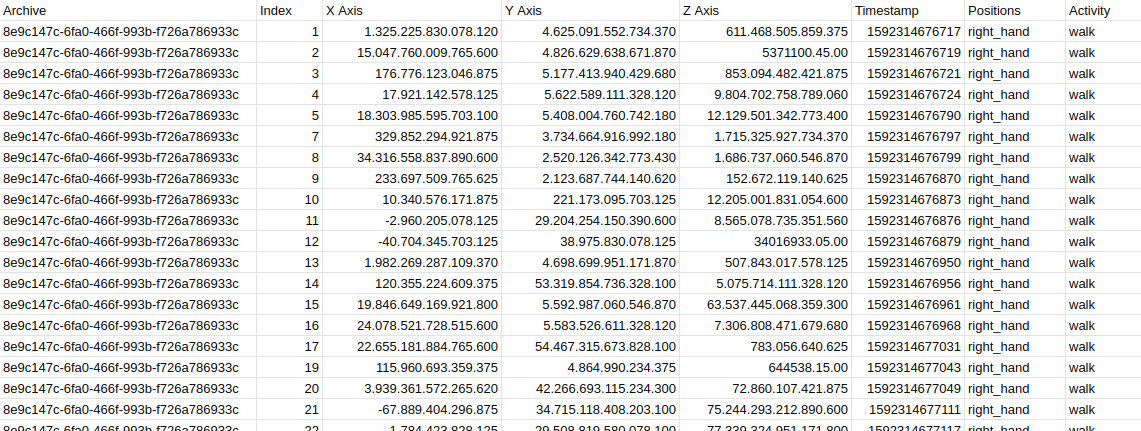
\includegraphics[scale = 0.39]{assets/images/examples/dataset-data-example.png}
    \caption{Esempio del dataset CSV contenente dati accelerometrici}
    \label{fig:example-dataset-csv-accelerometer}
\end{figure}


\subsubsection{Messaggi di Analisi}
Nel caso di ricezione di dati per l'analisi non si deve immagazzinare passivamente tutte le informazioni ricevute, ma è necessario fornire
al client connesso le risposte che si aspetta.

Alla ricezione del numero minimo di record si avvia il processo di predizione del classificatore, trattato sempre nel capitolo \ref{chapter:classification}.
Una volta ottenuta l'ipotesi, questa sarà inviata come risposta in formato JSON.

\begin{listing}[H] 
    \inputminted[frame=single,framesep=10pt]{json}{assets/snippets/server/receiver/prediction.json}
    \caption{Esempio di messaggio di risposta con l'ipotesi formulata}
\end{listing}